% IMPORTS, ETC %%%%%%%%%%%%%%%%%%%%%%%%%%%%%%%%%%%%%%%%%%%%%%%%%%%%%%%%%%%%%%%%%%%%%%%%%%%%%%%%%%%%%%%%
\documentclass[11pt, a4paper, twocolumn]{article}
\usepackage[english]{babel}

\usepackage{verbatim} %For code

\usepackage{array} %Tables
\newcolumntype{C}[1]{>{\centering\let\newline\\\arraybackslash\hspace{0pt}}m{#1}} %Center a fixed-size cell

\usepackage{color}
\definecolor{myblue}{RGB}{0, 100, 140} %References in color

\renewcommand{\labelitemi}{$\textendash$} %Change label of list item

%Page borders
\usepackage[a4paper, total={6in, 8in}]{geometry}
\setlength{\columnsep}{3em}

% PAPER INFO %%%%%%%%%%%%%%%%%%%%%%%%%%%%%%%%%%%%%%%%%%%%%%%%%%%%%%%%%%%%%%%%%%%%%%%%%%%%%%%%%%%%%%%%

\title{Dedicated test classes vs dependency injection}
\author{Irati Casi}
\date{\today}

\usepackage{graphicx}
\graphicspath{{images/}}

\makeatletter
\let\thetitle\@title
\let\theauthor\@author
\let\thedate\@date
\makeatother

\begin{document}

% TITLE PAGE %%%%%%%%%%%%%%%%%%%%%%%%%%%%%%%%%%%%%%%%%%%%%%%%%%%%%%%%%%%%%%%%%%%%%%%%%%%%%%%%%%%%%%%%

\begin{titlepage}
	\centering
    \vspace*{2 cm}
    
\includegraphics[scale = 0.25]{tu-delft.png}\\[1.0 cm]
    \textsc{\LARGE Delft University of Technology}\\[2.0 cm]
	\textsc{\Large Computer Science}\\[0.5 cm]
	\textsc{\large Bachelor thesis}\\[0.5 cm]
	\rule{\linewidth}{0.2 mm} \\[0.4 cm]
	{ \huge 
	\bfseries 
	\thetitle}\\
	\rule{\linewidth}{0.2 mm} \\[1.5 cm]
	
	\begin{minipage}{0.4\textwidth}
		\begin{flushleft} \large
			\emph{Author:}\\
			\theauthor
			\end{flushleft}
			\end{minipage}~
			\begin{minipage}{0.4\textwidth}
			\begin{flushright} \large
			\emph{Supervisor:} \\
			Mauricio Aniche	
		\end{flushright}
	\end{minipage}\\[2 cm]
	
	{\large \thedate}\\[2 cm]
 
	\vfill
	
\end{titlepage}

% INTRO %%%%%%%%%%%%%%%%%%%%%%%%%%%%%%%%%%%%%%%%%%%%%%%%%%%%%%%%%%%%%%%%%%%%%%%%%%%%%%%%%%%%%%%%
\begin{abstract}
This document is an analytical research about the relationship between the use of the dependency injection principle and the use of unit testing in object-oriented programming. Source code and javadoc of the tool is available on https://github.com/iraticasi/testability2.0 a
\end{abstract}


\section{Introduction}
In today’s business world, software is everywhere and its quality is becoming fundamental. Along with this, the knowledge of the importance and benefits of software testing is increasing. Testing not only improves the quality of the software but also helps measuring its reliability. With this in mind, now we should pay attention to what makes our code easier to test.\\
As each project is unique, there is no such thing as "the best method for testing". However, software testing best practices can ease our work. Several researches have been made about this topic and testing experts have shared their insights.\\
Dependency injection is said to improve testing since it enables mock practice to perform testing in isolation. This paper aims to discover whether the assertion holds. For this purpose, an analysis of various java projects will be performed in search of a relationship between the use of the principle and how the class is being tested.


% BACKGROUND %%%%%%%%%%%%%%%%%%%%%%%%%%%%%%%%%%%%%%%%%%%%%%%%%%%%%%%%%%%%%%%%%%%%%%%%%%%%%%%%%%%%

\section{Background} \label{background}
\begin{description}
\item [Dependency Injection Principle] in object-oriented programming is a design principle whereby objects are supplied to a class, instead of being created inside the class.\\
A simple example of a class that does not follow the principle could be:
\begin{verbatim}
class A{	
   B b;
   A(){
      this.b = new B();
   }
}
\end{verbatim}
And the alternative using dependency injection is the following:
\begin{verbatim}
class A{	
   B b;
   A(B b){
      this.b = b;
   }
}
\end{verbatim}
\item [Mock objects] simulate the behavior of real objects. They are usually created to test some other object in isolation. In a unit test, mock objects can simulate the behavior of complex, real objects and are therefore useful when a real object is impractical or impossible to incorporate into a unit test. 
\item [Testability] can be defined as \textit{“the degree to which a software artifact supports testing in a given test context”}. It involves two components: the effort and effectiveness of software tests .
\end{description}
When objects are not created inside the class, mock objects can be injected. Therefore, it is reasonable to believe that dependency injection simplifies unit testing. 


% RELATED WORK %%%%%%%%%%%%%%%%%%%%%%%%%%%%%%%%%%%%%%%%%%%%%%%%%%%%%%%%%%%%%%%%%%%%%%%%%%%%%%%%%%%%%%%%


\section{Related work}
As mention in section 1, we can find testing good practice that has been shared on the internet. In 2008, Google shared a guide to write testable code \cite{testablecode} that mentions 4 flaws: "Constructor does Real Work", "Digging into Collaborators", "Brittle Global State \& Singletons" and "Class Does Too Much". It also provides warning signs and alternatives.

There are also several researches about how different factors affect testability: 
{\color{myblue} Gao, J., Gupta, K., Gupta, S., \& Shim, S. (2002)} \cite{testablecomponents} focus on how to build testable software components by increasing their testability ;
{\color{myblue} Bruntink, M., \& van Deursen, A. (2006)}  \cite{classtestability} investigate testability factors in object-oriented software systems; 
{\color{myblue} Voas, J., \& Kassab, L. (1999)} \cite{assertions} study the effects of assertions;
{\color{myblue} Ma, L., Zhang, C., Yu, B., \& Sato, H. (2015)} \cite{visibility} analyze the influence of code visibility...

Some researchers focus on dependency injection effects: 
{\color{myblue} Yang, H. Y., Tempero, E., \& Melton, H. (2008)} \cite{dependencyjava} examine the use of dependency injection and its impact in software quality attributes such as extensibility, modifiability, testability and reusability; 
{\color{myblue} Razina, E., \& Janzen, D. S. (2007)} \cite{maintainability} study its effects on maintainability...\\
{\color{myblue} Mengkeang Veng (2014)} \cite{dependency} studies the effects of dependency injection and mocking on software and testing and attempt to answer four research questions: To what extent does dependency injection improve code structure design? To what extent does dependency injection facilitate software testing? To what extent does mock facilitate software testing? And to what extent do dependency injection and mock facilitate software testing. In order to answer those questions, an experiment is carried out in which two systems are compared to measure the extent of facilitation of the dependency injection on software. The results demonstrate that the dependency injection does not seem to improve the code design if comparing on the selected metrics and that the testability of the two systems is similar.


% METHODOLOGY %%%%%%%%%%%%%%%%%%%%%%%%%%%%%%%%%%%%%%%%%%%%%%%%%%%%%%%%%%%%%%%%%%%%%%%%%%%%%%%%%%%%%%%%

\section{Methodology}
In order to discover if dependency injection improves testability, the study will collect various projects and analyze their classes in search of a relationship between following the principle and how they are being tested. Our hypothesis is that classes that follow the DIP are better tested in isolation than those classes that do not.\\ 
This can be called a "analytical research" in which the researcher has to use facts or information already available and analyze them to make a evaluation of the material.\\
To reach the overall goal, three main research decisions can be identified: 
\begin{enumerate}
\item How to measure the use of dependency injection in a class.
\item How to measure in which degree a class is being tested in isolation.
\item How to collect the projects.
\end{enumerate}
In the following subsections, each decision will be covered one by one.

\subsection{DIP use measurement}
As mention in section \ref{background}, a class that follows the DIP instead of creating the objects, get the instances passed as parameters. Thus, in order to measure the use of this principle, we need to analyze creations of objects and to this effect, we need to detect the \texttt{new} keyword.  In this paper, we are going to refer to these creations as "dependencies".
\begin{description}
\item ["Dependency"] is a creation of an object inside a class. So if an object B is created inside class A, class A depends on class B.
\end{description}
Among all the dependencies, there are some that can not be consider to violate the DIP. These include some trivial java dependencies like lists, sets or dates from the \texttt{java.util} package. Besides, dependencies of the same package are under our control (unless these classes violate the DIP), so we are not going to consider those either. Now, we can classify these exceptions as "internal dependencies" and the rest as "external dependencies".
\begin{description}
\item ["External dependency"] is a dependency on:
\begin{itemize}
\item a class that is neither from the same package nor from \texttt{java.util}
\item a class that has external dependencies itself (recursive)
\end{itemize}
\item["Internal dependency"] is a dependency that is not "external".
\end{description}
Similarly, we can define "external classes" and "internal classes":
\begin{description}
\item ["External class"] is a class with external dependencies. Thus, it violates the DIP.
\item["Internal class"] is a class without external dependencies. Thus, it follows the DIP.
\end{description}

\subsection{Testing measurement}
The next decision is how to measure in which degree a class is being tested in isolation. Among all the test, we are interested in unit tests since they are those that are supposedly improved by the use of the DIP. For this measure, we propose two metrics.

\begin{itemize}
\item \textbf{If the class has a dedicated unit test class.} By convention, the unit test classes are named with the name of the class to be tested followed by the suffix "Test" or "Tests". An easy way to check if a class has a unit test is to search for a class with that format. That is why we are going to consider a class to have a dedicated test if there exists a class named \verb+<classname>Test.java+ or \verb+<classname>Tests.java+.\\
\item \textbf{The code coverage of the class.} This metric would be more precise, since the existence of a dedicated test does not necessarily mean that the class is being properly tested. There are different tools available that allow us to register the number of lines executed while testing, some of them integrate easily with maven.
\end{itemize}
In this research, only the first metric is implemented, but the idea is to extend it with code coverage as we discuss in section \ref{conclusion}.\\

\subsection{Collect projects}
If we want to collect projects in an easy and cheap way, our best option is Github. Github counts with millions of open source projects in multiple programming languages. But how can we select a few projects between millions? Our idea is to obtain them from \textit{The Apache Software Foundation}, since it counts with hundreds of open source well-know projects. Besides, many of them are written in Java and all of them use Maven, which will be convenient for future analysis of the code coverage.\\


% IMPLEMENTATION %%%%%%%%%%%%%%%%%%%%%%%%%%%%%%%%%%%%%%%%%%%%%%%%%%%%%%%%%%%%%%%%%%%%%%%%%%%%%%%%%%%%%%%%

\section{Implementation}
Once it has been defined how to measure the use of DIP and the degree in which a class is being tested and how to collect the projects, we can implement the tool. The tool is written in java in the package \texttt{com.github.iraticasi.testability} and it is divided in three subpackages:
\begin{description}
\item[\texttt{analyzer}] provides analysis for the use of the dependency injection principle.
\item[\texttt{report}] contains implementation for report generation about the correlation between the use of dependency injection and testing.
\item[\texttt{collector}] provides a apache project collector.
\end{description}
In the following subsections, each package will be briefly explained. For more specific information, you can take a look to the javadoc or the source code.

\subsection{Analyzer package}
This package counts with two classes:
\begin{description}
\item[\texttt{Analyzer}]: instances can be constructed from the directory of a project.\\
Its method \texttt{analyze()} analyze the project and return a list of \texttt{ClassInfo}.\\
Its method \texttt{makeReport(String file)} create a CSV report named \verb+<file>+ with the format shown in Table \ref{table:external}.

\begin{table}[b] \centering
\begin{tabular}{ | m{4.5em} | m{4.5em}| m{6em} |}
\hline Package & Class & External dependencies \\ 
\hline \texttt{package name} & \texttt{class name} & Y/N\\
\hline \ldots & \ldots & \ldots \\
\hline
\end{tabular}
\caption{Format of external dependencies report}
\label{table:external}
\end{table}

\item[\texttt{ClassInfo}]: It represents a class of the project and holds all the required information that can be obtained using the methods: \texttt{getName()}, \texttt{getPkg()}, \texttt{getDependencies()} and \texttt{hasExternalDependencies()}.
\end{description}

\subsection{Report package}
The class \texttt{TestChecker} is responsible for generating reports with statistics of the existence of dedicated tests. An instance of this class can be created from a folder with the target projects and it includes two public methods:
\begin{description}

\item{\texttt{externalReport(String file)}} creates a CSV report of external dependencies. For each project, it computes statistics of the relationship between classes with external dependencies and classes with dedicated test. The report follows the format shown in Table \ref{table:external_test} and its fields are explain after that.

\begin{table*}[t] \centering
\begin{tabular}{ | m{5em} | m{8em} | m{8em} | m{7.5em} | m{7.5em} |}
\hline Project name & \# external classes with tests & \# external classes without tests & \# internal classes with tests & \# internal classes with tests \\
\hline \ldots & \ldots & \ldots & \ldots & \ldots \\
\hline
\end{tabular}
\caption{Format of test and external dependencies correlation report.}
\label{table:external_test}
\end{table*}

\begin{itemize}
\item \textit{Project name}: The name of the analyzed project.
\item \textit{\# external classes with test}: Number of "external" classes that have a dedicated test.
\item \textit{\# external classes without test}: Number of "external" classes that do not have a dedicated test.
\item \textit{\# internal classes with test}: Number of "internal" classes that have a dedicated test.
\item \textit{\# internal classes without test}: Number of "internal" classes that do not have a dedicated test.
\end{itemize}


\begin{table*}[t] \centering
\begin{tabular}{ | m{5em} | m{7em} | m{7em} | m{7em} | m{7em} |}
\hline Library name & library dep with test & library dep without test & no library dep with test & no Library dep no test\\
\hline \ldots & \ldots & \ldots & \ldots & \ldots \\
\hline
\end{tabular}
\caption{Format of test and libraries use correlation report.}
\label{table:libraries}
\end{table*}

\item{\texttt{librariesReport(String file, String[] libraries)}} is implemented to generate a report that shows the relation between a class having dependencies on some given libraries and having a dedicated test. This functionality is not used in this research, it is only implemented for future work as discussed in section \ref {conclusion}. The report follows the format shown in Table \ref{table:libraries} and its fields are explain hereunder:
\begin{itemize}
\item \textit{Library name}: The name of the library.
\item \textit{Library dep with test}: Number of classes that have dependencies on classes of that library and a dedicated test.
\item \textit{Library dep without test}: Number of classes that do not have dependencies on classes of that library but have with a dedicated test.
\item \textit{No library dep with test}: Number of classes that do not have dependencies on classes of that library nor a dedicated test.
\item \textit{No library dep without test}: Number of classes that does not have dependencies on classes of that library but have a dedicated test.
\end{itemize}


\end{description}

\subsection{Collector package}
This package is only created in order to collect projects automatically using the github API. The class \texttt{ProjectorCollector} clones a given number of apache projects written in java in the folder \verb+apache_projects+.

% RESULTS %%%%%%%%%%%%%%%%%%%%%%%%%%%%%%%%%%%%%%%%%%%%%%%%%%%%%%%%%%%%%%%%%%%%%%%%%%%%%%%%%%%%%%%%

\section{Results}
The analysis has been carried out for 18 projects with a total of 29,013 classes, the resulting report is shown in \textbf{table \ref{table:report}}.\\
\subsection{Results by project}
\textbf{Figure \ref{fig:dip}} represents the dependency injection use per project. The percentage of classes that follow the principle goes from 19\% (\texttt{beam}) to a maximum of 53\% (\texttt{incubator-skywalking}). We can observe for example that 27\% of \texttt{flink} classes and 24\% of cassandra classes follow the principle.\\
\textbf{Figure \ref{fig:withtest}} represents the use of dedicated test per project. The percentage of classes that have a dedicated test goes from 0.1\% (\texttt{hive}) to 44\% (\texttt{beam}). If we focus on the projects mentioned above, 24.6\% of \texttt{flink} classes and 19.9\% of cassandra classes have a dedicated test.\\
\textbf{Figure \ref{fig:dip_withtest}} shows the percentages of classes that count with a dedicated test per project differentiating external and internal classes. Red bars show the percentage of external classes with tests and green bars show the percentage of internal classes with tests. For example, in \texttt{flink} 28.8\% of  external classes and 13.2\% of internal classes have a dedicated test. Contrary to what we expect, in every project the percentage of external classes that have a dedicated test is greater than the percentage of internal classes that have a dedicated test.\\
\subsection{Overall results}
Lastly, in \textbf{table \ref{table:total}} we have the external report overall results. Only 12.2\% of classes have a dedicated test and 29.7\% follow the dependency injection principle according to our definition.\\
\textbf{Figure \ref{fig:dip_withtest_overall}} shows that 14.99\% of external classes and only 5.74\% of internal classes have a dedicated test.

% DISCUSSION %%%%%%%%%%%%%%%%%%%%%%%%%%%%%%%%%%%%%%%%%%%%%%%%%%%%%%%%%%%%%%%%%%%%%%%%%%%%%%%%%%%%%%%%

\section{Discussion}
Our hypothesis was that classes that follow the DIP are better tested in isolation than those classes that do not. Therefore, we thought that the percentage of internal classes that have a dedicated test was going to be greater than the percentage of external classes that have a dedicated test. Unexpectedly, results show the opposite. They also show a low use of unit testing and dependency injection according to our definition .\\
Unit testing finds problems early in the development cycle, facilities changes and simplifies integration, but the tests can be more complex than the actual code \cite{waste}. Thus, we conjecture that developers decide to focus on integration testing. \\
On the other hand, interdependence between classes is unavoidable. Coupling of object implementations is not always bad and sometimes is better to create a dependency in the dependent class than to code the loosely-coupled resolution of the dependency (injection, service location, factory). That can be a the reason why so few classes follow the principle.
Yet, the assumptions made above do not explain why "external classes" are slightly more tested so we have come to the following suppositions:
\begin{itemize}
\item A significant proportion of classes that have no dependencies are simple by nature so developers do not create unit test for them.
\item Apart from java.util and classes from the same package, there might be other classes that we did not consider that should not be injected either.
\end{itemize}
% CONCLUSION %%%%%%%%%%%%%%%%%%%%%%%%%%%%%%%%%%%%%%%%%%%%%%%%%%%%%%%%%%%%%%%%%%%%%%%%%%%%%%%%%%%%%%%%


\section{Conclusion} \label{conclusion}
We have perform an analysis in search of a relationship between the use of DI and the use of unit testing. The obtained results indicate a low use of both DIP and unit testing and, contrary to what we expected, that classes that follow the principle are slightly more tested.\\
For future work, code coverage will make a more accurate analysis and will provide us a better understanding of unit testing use. Another approach would be try to detect which libraries dependencies make classes that have them be less testable. Using the library report of the \texttt{report} package, you can analyze the existence of dedicated test in classes that have dependencies on a given library.

% REFERENCES %%%%%%%%%%%%%%%%%%%%%%%%%%%%%%%%%%%%%%%%%%%%%%%%%%%%%%%%%%%%%%%%%%%%%%%%%%%%%%%%%%%%%%%%

\begin{thebibliography}{00}

%%% GOOD PRACTICE

\bibitem{testablecode} 
Jonathan Wolter, Russ Ruffer, Miško Hevery (2008).
\textit{Guide: Writing Testable Code}. 

\bibitem{testablecomponents}
Gao, J., Gupta, K., Gupta, S., \& Shim, S. (2002, February).
\textit{On building testable software components}.
In International Conference on COTS-Based Software Systems (pp. 108-121). Springer, Berlin, Heidelberg.


%%%% EFFECTS ON TESTABILITY

\bibitem{classtestability}
Bruntink, M., \& van Deursen, A. (2006). 
\textit{An empirical study into class testability}.
Journal of systems and software, 79(9), 1219-1232.

\bibitem{assertions}
Voas, J., \& Kassab, L. (1999).
\textit{Using assertions to make untestable software more testable}.
Software Quality Professional, 1(4), 31.

\bibitem{visibility}
Ma, L., Zhang, C., Yu, B., \& Sato, H. (2015, May).
\textit{An empirical study on effects of code visibility on code coverage of software testing}.
In Automation of Software Test (AST), 2015 IEEE/ACM 10th International Workshop on (pp. 80-84). IEEE.


%%%% DEPENDENCY EFFECTS

\bibitem{dependencyjava}
Yang, H. Y., Tempero, E., \& Melton, H. (2008, March).
\textit{An empirical study into use of dependency injection in java. In Software Engineering, 2008}.
ASWEC 2008. 19th Australian Conference on (pp. 239-247). IEEE.

\bibitem{maintainability} 
Razina, E., \& Janzen, D. S. (2007). 
\textit{Effects of dependency injection on maintainability.}
In Proceedings of the 11th IASTED International Conference on Software Engineering and Applications: Cambridge, MA (p. 7).

\bibitem{dependency} 
Mengkeang Veng (2014).
\textit{Dependency Injection and Mock on Software and Testing}. 
Master thesis, Department of Informatics and Media,  Uppsala University.

\bibitem{waste} 
James O Coplien (2014).
\textit{Why Most Unit Testing is Waste}. 
RBCS.



\end{thebibliography}



\begin{table*}[] \centering
\begin{tabular}{ | m{7em} | C{7em} | C{7em} | C{7em} | C{7em} |}
\hline \textbf{Project name } & \textbf{\# external classes with tests} & \textbf{\# external classes without tests} & \textbf{\# internal classes with tests} & \textbf{\# internal classes without tests}  \\
\hline incubator-weex       & 45		& 597       & 8		& 230 	\\
\hline hive                 & 2		& 4133		& 3    	& 1339 	\\
\hline zeppelin             & 112	& 195       & 9		& 115  	\\
\hline rocketmq             & 80		& 230      	& 13		& 266  	\\
\hline zookeeper            & 52		& 201      	& 14   	& 109  	\\
\hline jmeter               & 35		& 718		& 4     & 332  	\\
\hline groovy               & 51		& 733       & 10		& 428  	\\
\hline tomcat               & 3		& 1284     	& 0     & 675  	\\
\hline incubator-dubbo      & 194	& 285  		& 53		& 279	\\
\hline kafka                & 334	& 433		& 32    	& 378	\\
\hline storm                & 152	& 1128		& 21    & 494	\\
\hline beam                 & 587	& 626		& 72		& 213	\\
\hline incubator-skywalking & 110	& 776		& 50    & 934	\\
\hline flink                & 870	& 2146		& 147	& 970	\\
\hline cordova-android      & 1		& 21			& 1     & 15		\\
\hline incubator-heron      & 125 	& 361		& 34		& 246	\\
\hline hbase                & 5    	& 2526		& 0     & 747  	\\
\hline cassandra            & 299   	& 939		& 24		& 359 	\\
\hline 
\end{tabular}
\caption{External report results.}
\label{table:report}
\end{table*}




\begin{figure*}
    \centering
    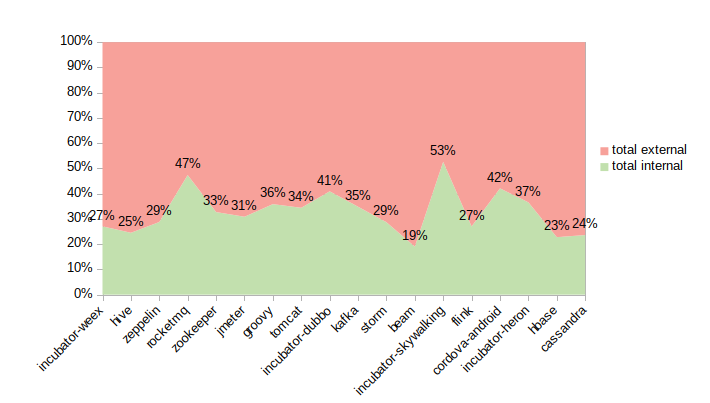
\includegraphics[scale = 0.75]{dipuse_plot.png}
    \caption{\textsf{Dependecy injection principle use.}}
    \label{fig:dip}
\end{figure*}

\begin{figure*}
    \centering
    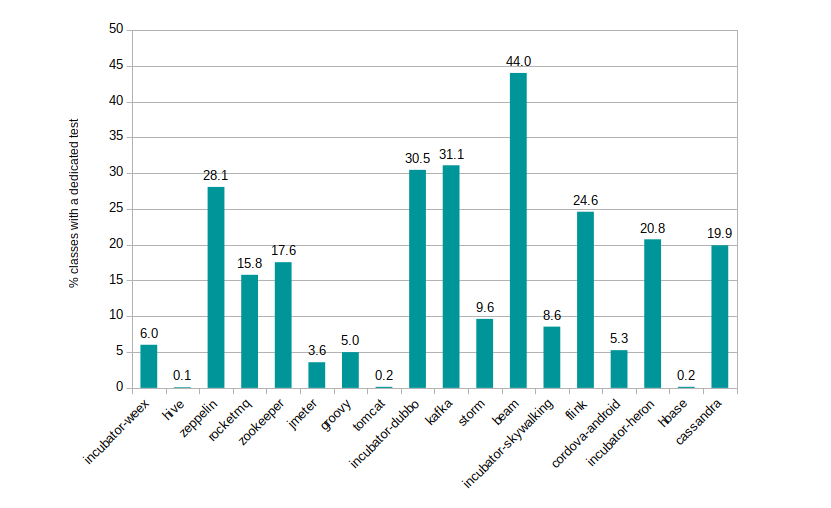
\includegraphics[scale = 0.7]{test_plot.png}
    \caption{\textsf{Use of dedicated test.}}
    \label{fig:withtest}
\end{figure*}

\begin{figure*}
    \centering
    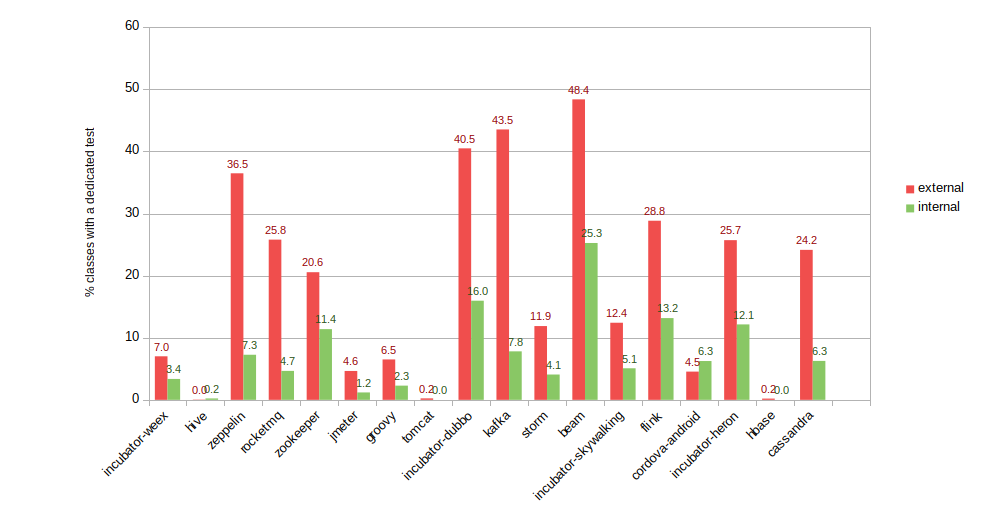
\includegraphics[scale = 0.6]{test_dipuse_plot.png}
    \caption{\textsf{Dependency injection principle use on external/internal classes per project.}}
    \label{fig:dip_withtest}
\end{figure*}

\begin{figure*}
    \centering
    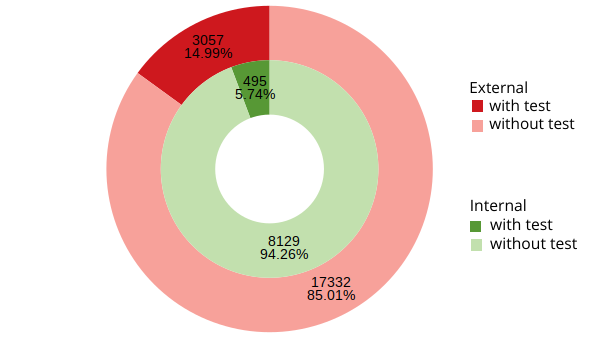
\includegraphics[scale = 0.6]{overall_plot.png}
    \caption{\textsf{Dependency injection principle use on all external/internal classes .}}
    \label{fig:dip_withtest_overall}
\end{figure*}

\begin{table*}[] \centering
\begin{tabular}{|l|c|c|c|}
\hline
\multicolumn{1}{|c|}{} & \textbf{external} classes & \textbf{internal} classes & total \\ \hline
\textbf{with} test 		& 3057     			& 495      			& 3552 (12.2\%)  \\ \hline
\textbf{without} test	& 17332    			& 8129     			& 25461 (87.8\%) \\ \hline
total      		& 20389 (70.3\%)    & 8624 (29.7\%)    & 29013 \\ \hline
\end{tabular}
\caption{External report overall results.}
\label{table:total}
\end{table*}



\end{document}